\section{Podmínky optimality}

\subsection{Kužel přípustných směrů}
Nechť $M \subseteq \R^n$ a $x \in M$.
\begin{itemize}
    \item Vektor $d \in \R^n$ se nazve přípustný směr množiny $M$ v bodě $x$, jestliže existuje $\delta > 0$ tak, že pro
    každé $\alpha \in (0, \delta]$ je $x + \alpha d \in M$.
    \item Množina $\F(M; x)$ všech přípustných směrů množiny $M$ v bodě $x$ se nazývá kužel přípustných směrů množiny
    $M$ v bodě $x$.
\end{itemize}
$\F(M; x) \not = \emptyset$.\\
Je-li $x \in \Int(M)$, pak $\F(M; x) = \R^n$.\\
Je-li $M$ konečná (neprázdná), pak $\F(M;x) = \bc{0}$ pro každé $x \in M$.

\subsection{Přípustné směry poklesu}
Mějme
\begin{enumerate}[(a)]
    \item Je-li $M = S(0; 1)$, pak $\F(M;x) = \bc{0}$ pro každé $x \in M$.
    \item Je-li $C = B(0; 1)$ a $\hat x = (1, 0)^T$, pak
    \[
        F(C; \hat x) = \bc{
            \begin{bmatrix}
                d_1 \\
                d_2
            \end{bmatrix} \in \R^2 \, \middle| \, d_1 < 0
        } \cup \bc{
            \begin{bmatrix}
                0 \\
                0
            \end{bmatrix}
        }
    \]
\end{enumerate}
(a) $M = S(0; 1) = \bc{x \in \R^2 \mid \| x\| = 1}$

Úvaha: Polopřímka z bodu $(1,0)$ projde maximálně $2 \times$ skrz kružnici.
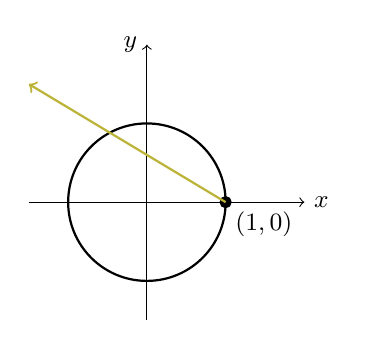
\begin{tikzpicture}
    \draw[thick] (0,0) circle(1);

    \draw[->] (-1.5,0) -- (2,0) node[right] {\small $x$};
    \draw[->] (0,-1.5) -- (0,2) node[left] {\small $y$};

    \filldraw (1,0) circle(2pt) node[below right] {\small $(1,0)$};

    \draw[thick,->, black!30!yellow] (1,0) -- (-1.5,1.5);
\end{tikzpicture}

Ať $d \not = 0 \in \R^2$
\[
    1 = \| x + \alpha d\|^2 = \langle x + \alpha d , x + \alpha d\rangle = \underbrace{\| x\|^2}_{1} + 2 \alpha
    \langle x, d\rangle + \alpha^2 \|d\|^2
\]
\[
    \rightarrow 0 = \alpha (2 \langle x, d\rangle + \alpha \| d\|^2) \implies \alpha =
    - \frac{2 \langle x,d\rangle}{\|d\|^2} \implies \F(M;x) = \bc{0}
\]

(b) Uvažujme kouli \\
$M = S(0; 1) = \bc{x \in \R^2 \mid \| x\| \leq 1}$; $x =
\begin{bmatrix}
    1 \\
    0
\end{bmatrix}$
\[
    1 \geq \left\|
    \begin{bmatrix}
        1 \\
        0
    \end{bmatrix} + \alpha d\right\|^2 = \left\langle
        \begin{bmatrix}
        1 \\
        0
    \end{bmatrix} + \alpha d ,
    \begin{bmatrix}
        1 \\
        0
    \end{bmatrix} + \alpha d\right\rangle = \underbrace{\left\|
    \begin{bmatrix}
        1 \\
        0
    \end{bmatrix}\right\|^2}_{1} + 2 \alpha
    \left\langle
    \begin{bmatrix}
        1 \\
        0
    \end{bmatrix}, d\right\rangle + \alpha^2 \|d\|^2
\]
\[
    \rightarrow 0 \geq \alpha (2 d_1 + \alpha \| d\|^2) \implies \alpha =
    - \frac{2 d_1}{\|d\|^2} \implies \F\left(M;
    \begin{bmatrix}
        1 \\
        0
    \end{bmatrix}\right) = \bc{
    \begin{bmatrix}
        d_1 \\
        d_2
    \end{bmatrix} \in \R^2 \, \middle| \, d_1 < 0
    }.
\]

\subsection{Kužel směrů poklesu}
Nechť $D \subseteq \R^n$, $x \in D$ a $f : D \rightarrow \R$.
\begin{itemize}
    \item Vektor $d \in \R^n$ se nazve směr poklesu funkce $f$ v bodě $x$, jestliže existuje $\delta >0$ tak, že pro
    každé $\alpha \in (0, \delta]$ je $f(x + \alpha d) < f(x)$.
    \item Množina $\D(f; x)$ všech směrů poklesu funkce $f$ v bodě $x$ se nazývá kužel směrů poklesu funkce $f$ v bodě
    $x$.
\end{itemize}
Definice implicitně obsahuje podmínku $[x, x+\delta d] \subseteq D$.

\subsection{Nutná geometrická podmínka lokálního extrému}
Jestliže $x$ je bod lokálního minima funkce $f : D \subseteq \R^n \rightarrow \R$ na $M \subseteq D$, pak
$\F(M; x) \cap D(f;x) = \emptyset$.

Důkaz. Sporem. \\
Ať ne, tj. existuje $d \in \F(M, x) \cap D(f, x)$.\\
Pak: $f (x + \alpha d) < f(x)$ a $x + \alpha d \in M$ pro všechna $\alpha > 0$ dostatečně malá.\\
Tedy spor s tím, že $x$ je bod lokálního minima $f$ na $M$. $\qed$

\subsection{Silný směr poklesu - linearisace směru poklesu}
Nechť $\Omega \subseteq \R^n$ je otevřená množina, $x \in \Omega$ a $f \in C^{1}(\Omega)$.
\begin{itemize}
    \item Vektor $d \in \R^n$ se nazve silný směr poklesu funkce $f$ v bodě $x$, jestliže $\langle \nabla f(x), d\rangle < 0$.
    \item Množina $\D_0(f; x)$ všech silných směrů poklesu funkce $f$ v bodě $x$ se nazývá kužel silných směrů poklesu
    funkce $f$ v bodě $x$.
\end{itemize}
Kužel $\D_0(f; x)$ je množina všech řešení lineární nerovnice \[\langle \nabla f(x), d\rangle < 0.\]
$\D_0(f;x)$ je konvexní kužel.

\subsection{Tvrzení o souvislosti přípustných směrů poklesu a jejich linearisaci}
Nechť $\Omega \subseteq \R^n$ je otevřená množina, $x \in \Omega$ a $f \in C^1(\Omega)$. Potom platí:
\begin{enumerate}[(a)]
    \item Je-li $d \in \D(f; x)$, potom $\langle \nabla f(x), d\rangle \leq 0$.
    \item $\D_0(f;x) \subseteq \D(f;x)$ (tj. jestliže $\langle \nabla f(x), d\rangle < 0$, pak $d \in \D(f;x)$).
\end{enumerate}
Důkaz.\\
(a) Ať $d \in D(f;x)$.
\[
    \frac{f(x + \alpha d) - f(x)}{\alpha} < 0 \text{ pro } \alpha > 0 \text{ dostatečně malé.}
\]
\[
    \implies \underbrace{\lim_{x\rightarrow 0^+ } \frac{f(x+\alpha d) - f(x)}{\alpha}}_{= \langle \nabla f(x), d\rangle}
    \leq 0 \qed
\]
\newpage
(b) Ať $\alpha > 0$.
\[
    f(x+\alpha d) = f(x) + \alpha \langle \nabla f(x), d\rangle + \alpha \| d\|
    \overbrace{\omega (\alpha d)}^{\text{zbytek}}
\]
\[
    \frac{f(x+\alpha d) - f(x)}{\alpha} = \underbrace{\langle \nabla f(x), d\rangle + \| d\| \omega (\alpha d)}_{
    \substack{\rightarrow \langle \nabla f(x), d\rangle \text{ pro } \alpha \rightarrow 0^+ \\ \text{a navíc }
    \langle\nabla f(x), d \rangle < 0}} \implies \frac{f(x + \alpha d) - f(x)}{\alpha} < 0
    \text{ pro všechna } \alpha < 0 \text{ dostatečně malá.}
\]

\subsection{Fermatova věta - nutná podmínka optimality}\label{fermat}
Nechť $\Omega \subseteq \R^n$ je otevřená množina, $M \subseteq \Omega$ a $\hat x \in M$ je bodem lokálního minima
funkce $f \in C^1(\Omega)$ na $M$. Potom platí:
\begin{enumerate}[(a)]
    \item $\F(M; \hat x) \cap \D_0(f; \hat x) = \emptyset$ (tj. $\langle \nabla f(\hat x), d\rangle \geq 0$ pro všechny
    $d \in \F(M; \hat x)$).
    \item Jestliže $\hat x \in \Int(M)$, pak $\nabla f(\hat x) = 0$.
\end{enumerate}
Důkaz.\\
(a) Víme, že $\F(M; \hat x) \cap \D(f; \hat x) = \emptyset$.\\ \label{fermatA}
Pak:
\[
    \D_0 (f, \hat x) \subseteq D(f, \hat x) \implies \F(M; \hat x) \cap \D_0(f, \hat x) = \emptyset. \qed
\]
(Tj. $\langle \nabla f(\hat x), d\rangle \geq 0 \quad \forall d \in \F(M, \hat x)$)

(b)
\[
    \hat x \in \Int(M) \implies \F(M; \hat x) = \R^n \overset{\hyperref[fermatA]{(a)}}{\implies}
    \langle \nabla f(\hat x), d\rangle \geq 0 \quad \forall d \in \R^n
\]
Ať $d = - \nabla f (\hat x)$.
\[
    - \| \nabla f(\hat x)\|^2 \geq 0 \implies \nabla f(\hat x) = 0. \qed
\]

\subsection{Věta o nutných a postačujících podmínkách pro konvexní úlohu}\label{nutnePostacujiciKonv}
Nechť $\Omega \subseteq \R^n$ je otevřená množina, $f \in C^1 (\Omega)$ je konvexní na $C \subseteq \Omega$ a
$\hat x \in C$. Potom platí:
\begin{enumerate}[(a)]
    \item $\hat x \in \argmin_{x \in C} f(x)$ právě tehdy, když $\F(C; \hat x) \cap \D_0(f; \hat x) = \emptyset$.
    \item Předpokládejme, že $\hat x \in \Int(C)$. Pak $\hat x \in \argmin_{x \in C}f(x)$ právě tehdy, když
    $\nabla f(\hat x) = 0$.
\end{enumerate}
Důkaz.

(a)\\
\enquote{$\Rightarrow$}: Víme. Když máme bod minima, je určitě bodem lokálního minima $\implies$ průnik je prázdný.\\
\enquote{$\Leftarrow$}: Sporem.\\
Ať existuje $y \in C : \overbrace{f(y) < f(\hat x)}^{f(y) - f(\hat x) < 0}$.\\
Ať $d = y - \hat x (\not = 0) \in \F(C, \hat x)$.\\
Cíl: $d \in \F(C, \hat x) \cap \D_0(f, \hat x)$.

\[
    \underbrace{\hat x + \alpha}_{\hat x + \alpha (y- \hat x) = \alpha y + (1-\alpha) \hat x} \hspace*{-11.5mm}d \in C \quad \forall
    \alpha \in [0, 1] \text{ z konvexity } C.
\]
$f$ je konvexní na $C \iff f(\hat x) + \langle \nabla f(\hat x), \overbrace{y - \hat x}^{d}\rangle \leq f(y)$.
$\implies \langle \nabla f(\hat x), d\rangle \leq f(y) - f(\hat x) \underset{\text{z předp.}}{<} 0$.\\
To je ale spor, protože byl předpoklad, že průnik je prázdný. My jsme ale ukázali, že není. $\qed$

(b)\\
\enquote{$\Rightarrow$} Víme.

\enquote{$\Leftarrow$} Ať $\nabla f(\hat x) = 0$.\\
Pak $\langle \nabla f(\hat x), d\rangle = 0 \quad \forall d \in \R^n = \F (C; \hat x)$. Nemáme tedy žádný směr poklesu
$\overset{\hyperref[nutnePostacujiciKonv]{(a)}}{\implies} \hat x \in \argmin_{x \in C} f(x). \qed$

\subsection{Hledání bodu minima}
$f(x, y) = x^2 + 3y^2 - 2xy + x - 2y$

$\nabla^2 f(x, y) =
\begin{bmatrix}
    \phantom{-}2 & -2 \\
    -2 & \phantom{-}6
\end{bmatrix} \dots$ dle Sylvesterova kritéria je positivně definitní. \\
$\implies f $ je nutně (ryze) konvexní.

\[
    0 = \nabla f(x, y) =
    \begin{bmatrix}
        2x-2y + 1 \\
        6y - 2x -2
    \end{bmatrix} \rightarrow
    \begin{matrix}
    \phantom{-}2x - 2y = -1 \\
    -2x + 6y = \phantom{-}2
    \end{matrix} \rightarrow y = \frac{1}{4} \Rightarrow x = -\frac{1}{4}.
\]

\subsection{Věta o podmínkách optimality 2. řádu}\label{podOpt2}
Nechť $\Omega \subseteq \R^n$ je otevřená množina, $M \subseteq \Omega$, $\hat x \in \Int(M)$ a $f \in C^2 (\Omega)$.
Potom platí:
\begin{enumerate}[(a)]
    \item Jestliže $\hat x$ je bod lokálního minima funkce $f$ na $M$, pak $\nabla^2 f(\hat x)$ je positivně
    semidefinitní.
    \item Jestliže $\nabla f(\hat x) = 0$ a $\nabla^2 f(\hat x)$ je positivně definitní, pak $\hat x$ je bod ostrého
    lokálního minima.
\end{enumerate}
Důkaz vynecháme.

\subsection{Příklad použití věty o podmínkách optimality 2. řádu}
Je dána funkce
\[
    f(x, y) = \frac{1}{3}x^3 + \frac{1}{2}y^2 + xy + 2y.
\]
Určete lokální extrémy funkce.

\[
    0 = \nabla f(x, y) =
    \begin{bmatrix}
        x^2 + y \\
        y + x + 2
    \end{bmatrix} \rightarrow
    \begin{matrix}
        x^2 + y = 0 \\
        y + x + 2 = 0
    \end{matrix} \rightarrow x^2 - x - 2 = 0 \rightarrow (x+1)(x-2) = 0
\]
Podezřelé body jsou:
\begin{itemize}
    \item $x = -1 \implies y = -1$
    \item $x = 2 \implies y = -4$
\end{itemize}
\[
    \nabla^2 f(x, y) =
    \begin{bmatrix}
        2x & 1 \\
        1 & 1
    \end{bmatrix}
\]
$\nabla^2 f(-1, -1) =
\begin{bmatrix}
    -2 & 1 \\
    \phantom{-}1 & 1
\end{bmatrix} \dots$ dle Sylvesterova kritéria není positivně semidefinitní, není ani negativně semidefinitní, je
indefinitní. Dle věty \hyperref[podOpt2]{o podmínkách optimality 2. řádu} není lokálním minimem ani maximem.\\
$\nabla^2 f(2, -4) =
\begin{bmatrix}
    4 & 1 \\
    1 & 1
\end{bmatrix} \dots$ dle Sylvesterova kritéria je positivně definitní. V bodě $(2, -4)$ se tedy nachází (ostré) lokální
minimum, nikoliv však globální.

\subsection{Hledání bodu minima}
Nalezněte, pokud existují, všechny body minima funkce
\[f(x, y, z) = 2x^2 + y^2 + z^2 + xy - 2xz\]
\[
    \nabla^2 f(x, y, z) = 
    \begin{bmatrix}
        \phantom{-}4 & 1 & -2 \\
        \phantom{-}1 & 2 & \phantom{-}0 \\
        -2 & 0 & \phantom{-}2
    \end{bmatrix}
\]
\[
    \begin{rcases*}
        \det \nabla^2 f(x, y, z) =
        \begin{vmatrix}
            \phantom{-}2 & 0 & 0 \\
            \phantom{-}1 & 2 & 0 \\
            -2 & 0 & 2
        \end{vmatrix} = 2 
        \begin{vmatrix}
            2 & 1 \\
            1 & 2
        \end{vmatrix} = 6 >0 \\
        \begin{vmatrix}
            4 & 1 \\
            1 & 2
        \end{vmatrix} = 7 > 0\\
        \begin{vmatrix}
            4
        \end{vmatrix} = 4 > 0
    \end{rcases*} \text{positivně definitní} \implies f \text{ je ryze konvexní.}
\]
Protože $f$ je konvexní, body minima budou přesně stacionární body. A protože $f$ je ryze konvexní, tak bude mít právě 
jeden bod minima.

\begin{alignat*}{4}
    4&x &+ \;& y &- 2&z &=\; 0 &\quad \Rightarrow 2z + y = 0 \Rightarrow z = -2y \\
    &x &+ 2& y &  &  &=\; 0 &\quad \Rightarrow x = -2y \\
   -2&x &  &  &+ 2&z &=\; 0 &\quad \Rightarrow x = z
\end{alignat*}
Jediný bod minima je tedy očividně 
$
\begin{bmatrix}
    x \\
    y \\
    z
\end{bmatrix}=
\begin{bmatrix}
    0 \\
    0 \\
    0
\end{bmatrix}
$.

\subsection{Omezení ve tvaru nerovnosti - aproximace \texorpdfstring{$\F(M;\hat x)$}{F(M;x)}}
Ať $g_1, \dots, g_k$ jsou reálné funkce definované na množině $\Omega \subseteq \R^n$,
$M = \bc{x \in \Omega \mid g_1(x) \leq 0, \dots, g_k(x) \leq 0}$ a $x \in M$.
Označme si:
\begin{itemize}
    \item Množina $\I \left((g_i)_{i=1}^k;x\right)\coloneq \bc{i \in \bc{1, \dots, k} \mid g_i(x) = 0}$ se nazývá
    indexová množina aktivních omezení v bodě $x$.
    \item Jestliže $i \in \I \left((g_i)_{i=1}^k;x\right)$, pak $g_i(x) \leq 0$ se nazve \textbf{aktivní} omezení (ve
    tvaru nerovnosti) v bodě $x$.
    \item Jestliže $i \not\in \I \left((g_i)_{i=1}^k;x\right)$, pak $g_i(x) \leq 0$ se nazve \textbf{neaktivní} omezení
    (ve tvaru nerovnosti) v bodě $x$.
\end{itemize}
Poznámka. V textu dále se obvykle bude uvádět pouze $\I(x) = \bc{i \in \bc{1, \dots, k} \mid g_i(x) = 0}$. Když
přeindexujeme funkce $g_i(x)$, znamenalo by to něco jiného, proto se u $\I$ uvádí $\left((g_i)_{i=1}^k;x\right)$, ale my
většinou přeindexovávat nebudeme.

Definice.

Nechť $\Omega \subseteq \R^n$ je otevřená množina, $g_1, \dots, g_k \in C^1(\Omega)$, $x \in M$ a $M = \bc{x \in \Omega
\mid g_1(x) \leq 0, \dots, g_k (x) \leq 0}$. Definujme množinu
\begin{align*}
    \G \left( (g_i)_{i=1}^k; x\right) \coloneq& \bc{d \in \R^n \, \middle| \, \langle \nabla g_i(x), d \rangle \leq 0 \quad \forall i \in \I (x)} \\
    =& \bigcap_{i \in \I(x)} \bc{d \in \R^n \, \middle| \, \langle \nabla g_i (x), d\rangle \leq 0}
\end{align*}
jako aproximaci $\F(M; \hat x)$.

% TODO: nákres

\subsection{Příklad výpočtu \texorpdfstring{$\G$}{G} a \texorpdfstring{$\F$}{F}}
Je dána množina
\[
    M = \bc{(x, y)^T \in \R^2 \mid y - x^3 \leq 0, -y \leq 0}
\] a bod $\hat x = (0, 0)^T$. Určete množiny $\F(M; \hat x)$ a $\G((g_i)_{i=1}^k; \hat x)$.

\begin{multicols}{2}
    Nákres množiny.

    \begin{tikzpicture}
        \begin{axis}[
            axis lines=middle,
            axis on top,
            xlabel={$x$},
            ylabel={$y$},
            xmin=-1.2, xmax=2.2,
            ymin=-1.5, ymax=9,
            samples=100,
            domain=-1:2,
            thick,
            xticklabels={},
            yticklabels={}
        ]
            \addplot[name path=f, blue, thick, domain=0:2] {x^3} node[left] {$f(x) = x^3$};
            \path[name path=x] (0,0) -- (2,0);
            \addplot[gray!50, on background layer] fill between[of=f and x];
            \addplot[blue, thick, domain=-1.1:0] {x^3};
        \end{axis}
    \end{tikzpicture}

\columnbreak

    Výpočet $\F(M; \hat x)$.

    ? $0 + \alpha d \in M \quad \forall \alpha > 0$ dostatečně malé.
    \begin{flalign}
        \alpha d_2 - \alpha^3 d_1^3 &\leq 0 &\\
        - \alpha d_2 &\leq 0 \quad \forall \alpha > 0 \text{ dostatečně malé.}&
    \end{flalign}
    \begin{flalign*}
        (4) &\implies d_2 \geq 0 &\\
        (3) &\implies d_2 \leq \alpha^2 d_1^3 \quad \forall \alpha > 0 \text{ dostatečně malé.}&
    \end{flalign*}

\end{multicols}
$d_2 \geq 0 \implies d_1 \geq 0$ a protože to platí $\forall \alpha >0$ dostatečně malá, pak $d_2 = 0$, protože si můžu
vzít libovolné malé, tedy i limitně blízké nule, $\alpha$. \\
$\implies \F(M; (0, 0)) = \bc{
    \begin{bmatrix}
        d_1 \\
        0
    \end{bmatrix} \in \R^2 \, \middle| \, d_1 \geq 0}$.

Výpočet $G\left( (g_i)_{i=1}^k; \hat x\right)$.

Označme si $g_1(x, y) = y-x^3$ a $g_2(x, y) = -y$.\\
Pak: 
\[
    \begin{rcases*}
        \langle \nabla g_1(0), d \rangle = \left\langle 
        \begin{bmatrix}
            0 \\
            1
        \end{bmatrix},
        \begin{bmatrix}
            d_1 \\
            d_2
        \end{bmatrix}\right\rangle = d_2 \leq 0\\
        \langle \nabla g_1(0), d \rangle = \left\langle 
        \begin{bmatrix}
            \phantom{-}0 \\
            -1
        \end{bmatrix},
        \begin{bmatrix}
            d_1 \\
            d_2
        \end{bmatrix}\right\rangle = d_2 \geq 0
    \end{rcases*} d_2 = 0
\]
$\implies \G((g_1, g_2), (0, 0)) = \bc{
\begin{bmatrix}
    d_1 \\
    0    
\end{bmatrix} \, \middle| \, d_1 \in \R}$ $\rightarrow$ $\G$ je větší jak $\F$. 

Protože $\G$ je pouze aproximací $\F$, může a bude se stávat, že $\G$ bude větší jak $\F$.

Přidejme si další, fakticky zbytečnou, podmínku navíc.

$M = \{(x, y)^T \in \R^2 \mid \underbrace{y - x^3}_{g_1(x, y)} \leq 0, \underbrace{-y}_{g_2(x,y)} \leq 0, 
\underbrace{-x -y}_{g_3(x,y)} \leq 0\}$

\[
    \langle \nabla g_3(0), d\rangle = \left\langle 
    \begin{bmatrix}
        -1 \\
        -1
    \end{bmatrix},
    \begin{bmatrix}
        d_1 \\
        d_2
    \end{bmatrix}
    \right\rangle = -d_1 - \underbrace{d_2}_{=0} \leq 0 \implies -d_1 \leq 0
\]
$\implies \G((g_1, g_2, g_3), (0,0)) = \bc{
\begin{bmatrix}
    d_1 \\
    d_2    
\end{bmatrix} \mid d_1 \geq 0}$. Což odpovídá přesně množině $\F$.

Je tedy očividné, že $\G$ závisí na popisu množiny.

\subsection{Ukázka, že aproximací \texorpdfstring{$\F$}{F} lze zkazit prázdnost průniku}
Mějme optimalisační úlohu
\begin{align*}
    \text{minimalisujte } x + y \\
    \text{za podmínek } y - x^3 &\leq 0, \\
     - y &\leq 0.
\end{align*}
Pak
\begin{align*}
    \D_0(f; 0) &= \bc{d \in \R^n \mid \langle \nabla f(0), d\rangle < 0} \\
    &\hspace*{-1.8em}\underset{\nabla f(0) = (1, 1)}{=} \bc{
    \begin{bmatrix}
        d_1 \\
        d_2
    \end{bmatrix} \mid d_1 + d_2 < 0} \dots \text{ například } 
    \begin{bmatrix}
        -1 \\
        \phantom{-}0
    \end{bmatrix} \in \D_0(f; 0), \text{ ale } 
    \begin{bmatrix}
        -1 \\
        \phantom{-}0
    \end{bmatrix} \in \G(x)!
\end{align*}
Tedy $\G(\hat x) \cap \D_0(f; \hat x) \not= \emptyset$ $\implies$ nahrazením podmínek optimality můžeme zkazit prázdnost 
průniku, protože $\G$ může být větší jak $\F$.
\newpage
\section{KKT podmínky}
\subsection{Věta o nutných KKT podmínkách}\label{KKT}
Nechť $\Omega \subseteq \R^n$ je otevřená množina, $f, g_1, \dots, g_k \in C^1 (\Omega)$,
\[
    M = \bc{x \in \Omega \mid g_1(x) \leq 0, \dots, g_k(x) \leq 0}
\]
a $\hat x \in M$. Jestliže $\overline{\F(M; \hat x)} = \G(\hat x)$ a $\hat x$ je bod lokálního minima na $f$ na $M$, 
pak existuje ${(\mu_1, \dots, \mu_k)^T \in \R^k}$ tak, že 
\begin{align*}
    \nabla f(\hat x) + \Sigma_{i=1}^k \mu_i \nabla g_i(\hat x) &= 0, \\
    \mu_i g_i(\hat x) &= 0 \text{ pro všechna } i \in \bc{1, \dots, k}, \\
    \mu_i &\geq 0 \text{ pro všechna } i \in \bc{1, \dots, k}.
\end{align*}

Důkaz.

\begin{itemize}
    \item $\I(\hat x) = \emptyset \implies \hat x \in \Int(M) \implies \nabla f(\hat x) = 0$ z 
    \hyperref[fermat]{Fermatovy věty}. \\
    $\rightarrow$ volba $\mu_1 = \dots = \mu_k = 0$. Pak KKT podmínky splněny.
    \item $\emptyset \not= \I(\hat x) = \bc{1, \dots, l}$\\
    Víme, že máme bod lokálního minima ($\hat x$) $\underset{\text{\hyperref[fermat]{věta}}}
    {\overset{\text{\hyperref[fermat]{Fermatova}}}{\implies}} \F(M; \hat x) \cap \D_0(f; \hat x) = \emptyset$, \\
    tj. $\langle \nabla f(\hat x), d\rangle \geq 0 \quad \forall d \in \F(M; \hat x)$. 

    Teď chceme dokázat, že platí $\langle \nabla f(\hat x), d\rangle \geq 0 \quad \forall d \in \G(\hat x)$. 

    Protože $\overline{\F(M; \hat x)}$ koinciduje s $\G(\hat x)$ a ze spojitosti skalárního součinu plyne, že \\ 
    $\langle \nabla f(\hat x), d\rangle \geq 0 \quad \forall d \in \underbrace{\overline{\F(M; \hat x)}}_{\G(\hat x)}$.

    To tedy znamená $\langle \nabla f(\hat x), d\rangle \geq 0 \quad \forall d \in \G(\hat x)$. Z toho plyne, že
    neexistuje $d \in \R^n$, pro který platí:
    \begin{equation*}
        \settowidth{\mylen}{$\displaystyle \langle \nabla g_1(\hat x), d \rangle \leq {}$\,}
        \begin{aligned}
            \langle \nabla f(\hat x), d \rangle &< 0 \, \dots \text{ tj. } \langle -\nabla f(\hat x), d\rangle > 0 \\
            &\phantom{{}<{}}
            \hspace*{-\dimexpr\mylen+\nulldelimiterspace}
              \left.\begin{aligned}
                  \langle \nabla g_1(\hat x), d \rangle &\leq 0 \\
                  & \vdots \\
                  \langle \nabla g_l(\hat x), d \rangle &\leq 0
              \end{aligned}\right\}
              A^T d \leq 0, \text{ kde } A = (\nabla g_1(\hat x), \dots, \nabla g_l(\hat x))
        \end{aligned}
    \end{equation*}
    No a z \hyperref[farkas]{Farkasova lemma} tedy nutně platí: ex. $\mu = (\mu_1, \dots, \mu_l)^T \in \R^l_+ : 
    \underbrace{A \mu}_{\hspace*{-2em}\sum_{i=1}^l \mu_i \nabla g_i} = - \nabla f(\hat x)$.\\
    $\rightarrow$ volme dále $\mu_{l+1}, \dots, \mu_k = 0$. Pak
    \begin{align*}
        - \nabla f(\hat x) &= \sum_{i=1}^k \mu_i \nabla g_i(\hat x), \\
        \mu_i \nabla g_i(\hat x) &= 0 \text{ pro všechna } i \in \bc{1, \dots, k}, \\
        \mu_i &\geq 0 \text{ pro všechna } i \in \bc{1, \dots, k}.
    \end{align*}
    A to jsou přesně KKT podmínky. $\qed$
\end{itemize}

\subsection{Příklad použití KKT podmínek}
\begin{align*}
    \text{minimalisujte } &\underbrace{x + y}_{f(x,y)} \\
    \text{za podmínek } &\underbrace{x}_{g_1(x,y)} \geq 0, \\
    &\underbrace{y}_{g_2(x,y)} \geq 0.
\end{align*}
Určete KKT body.\\
$\nabla f(x, y) = 
\begin{bmatrix}
    1 \\
    1
\end{bmatrix}$, $\nabla g_1(x,y) = 
\begin{bmatrix}
    -1 \\
    \phantom{-}0
\end{bmatrix}$, $\nabla g_2(x,y) = 
\begin{bmatrix}
    \phantom{-}0 \\
    -1
\end{bmatrix}$.

KKT podmínky:
\begin{align*}
    1 + \mu_1 (-1) + \mu_2 (0)  &= 0 \quad \rightarrow \mu_1 = 1 \\
    1 + \mu_1 (0) +  \mu_2 (-1) &= 0 \quad \rightarrow \mu_2 = 1 \\
    \mu_1 (-x) &= 0 \\
    \mu_2 (-y) &= 0 \\
    \mu_1, \mu_2 &\geq 0
\end{align*}
Jediný KKT bod je tedy 
$\hat x = \begin{bmatrix}
    0 \\
    0
\end{bmatrix}$ a jedná se o bod minima.

\subsection{Příklad, že KKT podmínky vždy nenaleznou všechny body}
\begin{align*}
    \text{minimalisujte } &x \\
    \text{za podmínek } &x^2 + (y-1)^2 \leq 1, \\
    &x^2 + (y+1)^2 \leq 1.
\end{align*}

\begin{multicols}{2}
    Nákres.

    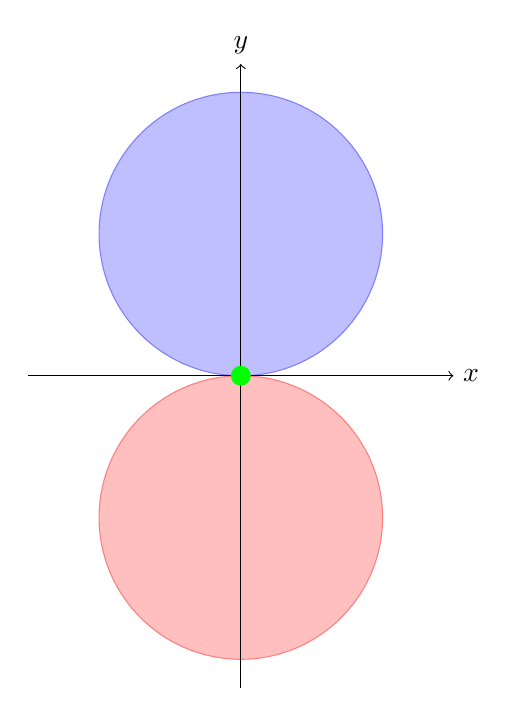
\begin{tikzpicture}[scale=1.8]
        \fill[blue!50, opacity=0.5] (0,1) circle (1);
        \fill[red!50, opacity=0.5] (0,-1) circle (1);
        
        \draw[blue!50] (0,1) circle (1);
        \draw[red!50] (0,-1) circle (1);
        
        \draw[->] (-1.5,0) -- (1.5,0) node[right] {$x$};
        \draw[->] (0,-2.2) -- (0,2.2) node[above] {$y$};

        \fill[green] (0,0) circle (2pt);
    \end{tikzpicture}
\columnbreak

    \textcolor{green}{Přípustná} množina: $M = \bc{0} \rightarrow$ určitě konvexní množina.

    KKT podmínky: 
    \begin{align*}
        1 + \mu_1 (2 \cdot 0) &+ \mu_2 (2 \cdot 0) = 0 \, \xmark \\
        &\vdots
    \end{align*}
    $\Rightarrow (0,0)$ není KKT bod i když je úloha konvexní a bod $(0,0)$ je očividně bodem minima.
\end{multicols}

\subsection{Věta o postačujících KKT podmínkách}
Nechť $\Omega \subseteq \R^n$ je otevřená množina, $f, g_1, \dots, g_k \in C^1(\Omega)$ jsou konvexní funkce na \\
$C = \bc{x \in \Omega \mid g_1(x) \leq 0, \dots, g_k(x) \leq 0}$. Jestliže $\hat x \in C$ je KKT bod, pak $\hat x$ je bod 
minima funkce $f$ na $C$.

Důkaz. Ať $x \ in C$. \\
Cíl: $f(x) - f(\hat x) \geq 0$ ($= \hat x$ je minimum)

Charakterisace pomocí tečné nadroviny: $f(\hat x) + \langle \nabla f(\hat x), x - \hat x\rangle \leq f(x) \quad x, 
\hat x \in C$

\[
    f(x) - f(\hat x) \underset{\substack{\text{$f$ je konvexní } \\ \text{na $C \subseteq \Omega$}} }{\geq} \langle 
    \nabla f(\hat x), x - \hat x\rangle \underset{\text{stacionarity}}{\overset{\text{podmínka}}{=}} \langle - \sum_{i=1}^{k} \mu_i \nabla g_i(\hat x), 
    x - \hat x\rangle
\]
\[
    = \sum_{i=1}^{k} - \langle \nabla g_i(\hat x), x - \hat x \rangle \mu_i = \sum_{i=1}^{n} (g_i(\hat x) - g_i(x)) \mu_i 
    \underset{\text{komplementarity}}{\overset{\text{podmínka}}{=}} - \sum_{i=1}^{n}    
    \underbrace{\mu_i}_{\substack{\text{podmínka}\\ \text{nezápornosti}}} \overbrace{g_i(x)}^{\leq 0 \, \forall x \in C}
    \geq 0. \qed
\]

\subsection{Afinní podmínka regularity}\label{afinniPodm}
Nechť $\Omega \subseteq \R^n$ je otevřená množina, $g_1, \dots, g_k \in C^1 (\Omega)$ a 
\[
    M = \bc{x \in \Omega \mid g_1(x) \leq 0, \dots, g_k(x) \leq 0}.
\]
Řekněme, že $(g_i)_{i=1}^k$ splňuje afinní podmínku regularity, jestliže $g_1, \dots, g_k$ jsou afinní.

\subsection{Slaterova podmínka regularity}\label{slaterPodm}
Nechť $\Omega \subseteq \R^n$ je otevřená množina, $g_1, \dots, g_k \in C^1 (\Omega)$ a 
\[
    M = \bc{x \in \Omega \mid g_1(x) \leq 0, \dots, g_k(x) \leq 0}.
\]
Řekněme, že $(g_i)_{i=1}^k$ splňuje Slaterovu podmínku regularity, jestliže $g_1, \dots, g_k$ jsou konvexní na $\Omega$
a existuje $x \in \Omega$ tak, že pro každé $i \in \bc{1, \dots, k}$ je $g_i(x) < 0$.

\subsection{Použití podmínek regularity k ověření KKT podmínek}
\begin{multicols}{2}
    \optAs{min}{2x^2 + y^2}{%
    x^2 + y^2 - 1 &\leq 0, \\
                -x &\leq 0.}
    \hyperref[afinniPodm]{Afinní podmínka} splněna není, \\ ověříme \hyperref[slaterPodm]{Slaterovu}.

\columnbreak

    \begin{figure}[H]
        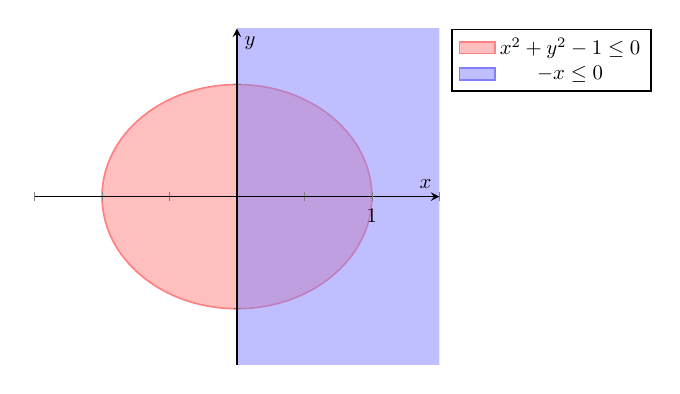
\begin{tikzpicture}[scale=0.75]
            \begin{axis}[
            axis lines=middle,
            axis on top,
            xlabel={$x$},
            ylabel={$y$},
            xmin=-1.5, xmax=1.5,
            ymin=-1.5, ymax=1.5,
            thick,
            xticklabels={},
            yticklabels={},
            extra x ticks={1},
            %legend pos=north west,
            %legend style={nodes={scale=0.5, transform shape}},
            legend pos=outer north east,
            ]
            \fill[red!50, opacity=0.5] (0,0) circle (1);
            \draw[red!50] (0,0) circle (1);
            \addlegendimage{area legend,red!50,fill=red!50,fill opacity=0.5}
            \fill[blue!50, opacity=0.5] (0,-2.5) rectangle (2.5,2.5);
            \addlegendimage{area legend,blue!50,fill=blue!50,fill opacity=0.5}
            \addlegendentry{$x^2+y^2-1\leq0$}
            \addlegendentry{$-x\leq0$}
            \end{axis}
        \end{tikzpicture}
    \end{figure}
\end{multicols}

Množina je očividně konvexní a zároveň zvolme $x = 
\begin{bmatrix}
    \frac{1}{2} \\
    0    
\end{bmatrix} \in \Omega$. Pak $g_i (x) < 0$, Slaterova podmínka je tedy očividně splněna.

$\nabla f (x) = 
\begin{bmatrix}
    4x \\
    2y    
\end{bmatrix}, \nabla g_1(x) =
\begin{bmatrix}
    2x \\
    2y
\end{bmatrix}, \nabla g_2(x) = 
\begin{bmatrix}
    -1\\
    \phantom{-}0
\end{bmatrix}$.

$\implies$ KKT podmínky:
\begin{align*}
    4x + \mu_1 2 x + \mu_2 (-1) &= 0 \leftrightarrow 2x (2+\mu_1) - \mu_2 = 0 \\
    2y + \mu_1 2 y + \mu_2 0    &= 0 \Leftrightarrow 2y (1+\mu_1) = 0 \underset{\mu_1 \geq 0}{\implies} y = 0 \\
    \mu_1(x^2 + y^2 - 1) &= 0 \\
    \mu_2(-x) &= 0 \\
    \mu_1, \mu_2 &\geq 0  
\end{align*}

$y=0$:
\[
    \begin{rcases*}
        2x(2+ \mu_1) = \mu_2 \\
        \mu_1(x^2 + 1) = 0 \\
        \mu_2 x = 0 \\
        \mu_1, \mu_2 \geq 0
    \end{rcases*}
    \begin{aligned}
        &x \not= 0 \Rightarrow \mu_2 = 0 \Rightarrow 2 + \mu_1 = 0 \dots \text{ spor s } \mu_1 \geq 0.\\
        &x = 0 \Rightarrow \mu_1 = 0 \Rightarrow \mu_2 = 0 \quad \checkmark
    \end{aligned}
\]

Existuje bod $
\begin{bmatrix}
x \\
y    
\end{bmatrix} =
\begin{bmatrix}
    0 \\
    0
\end{bmatrix}$, pro který jsou splněny nutné a postačující KKT podmínky.

\subsection{Určení nutných a postačujících podmínek optimality}
Ať $A \in \M_{m,n} (\R), \, D \in \M_{r,n}(\R), \, b\in \R^m$ a $\lambda > 0$. Je dána úloha
\[
    \text{minimalisujte } f(x) = \| Ax - b\|^2 + \lambda \| Dx\|^2  \text{ na } \R^n.
\]
Jaké jsou nutnné a postačující podmínky optimality?
\begin{align*}
    f(x) &= \langle Ax - b, Ax - b\rangle + \lambda \langle Dx, Dx\rangle \\
    &= \langle \underbrace{Ax, Ax}_{A^TAx, x}\rangle - 2\langle Ax, b\rangle + \| b\|^2 + \lambda \langle 
        \underbrace{Dx, Dx}_{D^TDx, x}\rangle
\end{align*}
$\implies f(x) = \left\langle \left(A^TA + \lambda D^TD\right)x, x\right\rangle - 2 \left\langle x, A^T b\right\rangle 
+ \| b\|^2$\\
Je $f$ konvexní?\\
Ano, neboť $\nabla^2 f(x) = 2(A^TA + \lambda D^TD)$ je positivně semidefinitní, protože pro $x \in \R$:
\begin{align*}
    \left\langle 2\left(A^TA + \lambda D^TD\right)x, x\right\rangle &= 2 \left[ \langle Ax, Ax\rangle + \lambda 
    \langle Dx, Dx\rangle\right] \\
    &= 2 \left[ \|Ax\|^2 + \lambda \|Dx\|^2\right] \geq 0
\end{align*}
Tedy $f$ je konvexní $\implies$ stačí najít stacionární body.
\begin{align*}
    0 = \nabla^2 f(x) &= 2 (A^TA + \lambda D^TD)x - 2(A^Tb) + 0 \\
    &= (A^TA + \lambda D^TD)x - A^Tb
\end{align*}
\[
    \implies A^Tb = (A^TA + \lambda D^TD)x
\]
A to je nutná a postačující podmínka pro $x$, aby byl bodem minima $f$ na $\R^n$.
    
\subsection{Určení KKT podmínek}
\begin{align*}
    \text{minimalisujte } &x^4 + y^4 + 12 x^2 + 6 y^2 - xy - x - y \\
    \text{za podmínek } &x + y \geq 6, \\
    &2x-y \geq 3, \\
    &x, y \geq 0.
\end{align*}
\begin{enumerate}[(a)]
    \item Napište KKT podmínky.
    \item Jsou nutné a postačující?
    \item Ukažte, že $(3, 3)^T$ je jediný bod minima.
\end{enumerate}
(a) Mějme
\begin{align*}
    g_1(x,y) &= -x-y+6, \\
    g_2(x,y) &= 2x-y+3, \\
    g_3(x,y) &= -x, \\
    g_4(x,y) &= -y, \\
    f(x,y) &= x^4 + y^4 + 12 x^2 + 6 y^2 - xy - x - y.
\end{align*}
$\rightarrow$ použijeme \hyperref[afinniPodm]{afinní podmínku regularity} $\rightarrow g_i$ jsou affiní.

KKT podmínky: 
\begin{align*}
    \nabla f(x, y) + \mu_1 \nabla g_1(x, y) + \mu_2 \nabla g_2(x, y) + \mu_3 \nabla g_3(x, y) + \mu_4 \nabla g_4(x, y) = 0 \\
    \mu_i g_i (x,y) = 0, i = 1,2,\dots,\\
    \mu_i \geq 0, i = 1,2,\dots.
\end{align*}
Tedy:
\begin{align*}
    4x^3 + 24x - y - 1 - \mu_1 - 2\mu_2 - \mu_3 = 0\phantom{,} \\
    4y^3 + 12y - x - 1 - \mu_1 + \mu_2 - \mu_4 = 0\phantom{,} \\
    \mu_1(-x-y+6) = 0, \\
    \mu_2(x-2y+3) = 0, \\
    x \mu_3 = 0, \\
    y \mu_4 = 0, \\
    \mu_1, \mu_2, \mu_3, \mu_4 \geq 0.
\end{align*}
Jsou postačující? Máme konvexní úlohu? Musíme ověřit konvexitu u $g_i$ a $f$.
\begin{itemize}
    \item $g_i$ jsou afinní $\implies$ jsou konvexní.
    \item $f:$
    \begin{itemize} % TODO: lepší argumentace
        \item kvadráty jsou ryze konvexní
        \item součet ryzích konvexních je ryzí konvexní
    \end{itemize} 
\end{itemize}
\[h(x, y) = 12x^2 + 6y^2 - xy -x -y\]
\[
    \nabla^2 h (x, y) = 
    \begin{bmatrix}
        \phantom{-}24 & -1 \\
        -1 & \phantom{-}12
    \end{bmatrix} = 24 \cdot 12 - 1 > 0; \quad 24 > 0 \implies h(x, y)\text{ je positivně definitní.}
\]
$\implies h(x, y)$ je ryze konvexní.

A proto je i $f(x, y)$ ryze konvexní, protože součet ryze konvexních dává ryze konvexní $\implies$ existuje právě jeden 
bod minima.\\
Ověříme $\begin{bmatrix} 3 \\ 3 \end{bmatrix}$. Ať $x=y=3$. Pak
\begin{align*}
    4 \cdot 27 + 24 \cdot 3 - 4 - \mu_1 + \mu_2 - \mu_3 = 0& \quad \text{(I.)} \\
    4 \cdot + 12 \cdot 3 - 4 - \mu_1 - 2\mu_2 - \mu_4 = 0& \quad \text{(II.)}\\
    \mu_1 \cdot 0 = 0& \\
    \mu_2 \cdot 0 = 0& \\
    3 \mu_3 = 0& \implies \mu_3 = 0\\
    3 \mu_4 = 0& \implies \mu_4 = 0\\
    \mu_1, \mu_2 \geq 0&
\end{align*}
I. $-$ II.: $24 \cdot 3 - 12 \cdot 3 - 3 \mu_2 = 0 \implies \mu_2 = \frac{1}{3} (24 \cdot 3 - 12 \cdot 3) > 0$.\\
$\mu_1 = 4 \cdot 27 + 24 \cdot 3 - 4 - \frac{2}{3}(24 \cdot 3 - 36) > 0$.

\subsection{Určení KKT podmínek}
\begin{align*}
    \text{minimalisujte } &\alpha x + y, \alpha \in \R \text{ je parametr.}\\
    \text{za podmínek } &x^2 + y^2 - 25 \leq 0, \\
    &x-y-1 \leq 0.
\end{align*}
Určete $\alpha$ tak, aby 
$\begin{bmatrix}
    4 \\
    3
\end{bmatrix}$ bylo řešení.

KKT podmínky:
\begin{align*}
    \alpha + \mu_1 (2x) + \mu_2 \cdot 1 = 0\phantom{,} \\
    1 + \mu_1 (2y) - \mu_2 = 0\phantom{,} \\
    \mu_1(x^2 + y^2 - 25) = 0, \\
    \mu_2(x - y - 1) = 0, \\
    \mu_1, \mu_2 \geq 0.
\end{align*}
$g_i$ jsou konvexní, $f$ je konvexní $\implies$ KKT podmínky jsou postačující.\\
\hyperref[slaterPodm]{Slaterova podmínka optimality} je splněna $\implies$ KKT podmínky jsou nutné.

$x=4, y=3$:
\begin{align*}
    \alpha + 8 \mu_1 + \mu_2 = 0& \quad \text{(I.)}\\
    1 + 6 \mu_1 - \mu_2 = 0&, \quad \text{(II.)}\\
    \mu_1, \mu_2 \geq 0&.
\end{align*}
I.+II.: $\alpha + 1 + 14 \mu_1 = 0$\\
$\mu_1 = \frac{-\alpha - 1}{14} \overset{!}{\geq} 0 \implies -1 \geq \alpha$. A tedy $\mu_2 = 1 + 6 \mu_1 \geq 0$.

Tedy aby
$\begin{bmatrix}
    4 \\
    3
\end{bmatrix}$ bylo řešení této úlohy, musí platit $\alpha \leq -1$.

\subsection{Určení KKT podmínek s trikem}
Mějme zadání
\begin{align*}
    \text{minimalisujte } \frac{x_1}{x_2} \\
    \text{za podmínek } &\frac{1}{x_1} + x_2 \leq 2, \\
    & x_1, x_2 > 0. 
\end{align*}

\begin{multicols}{2}
    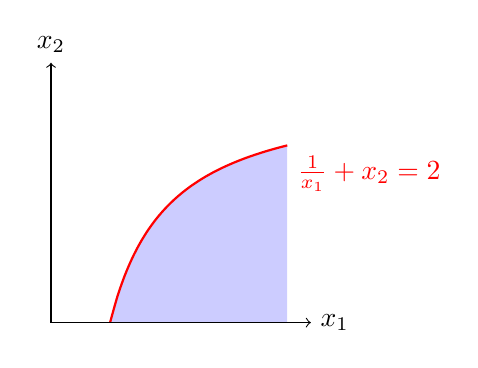
\begin{tikzpicture}[scale=1.5]
        \begin{scope}
            \clip (0,0) rectangle (2,2);
            \fill[blue!20] plot[domain=0.1:2] (\x, {2 - 1/(\x)}) -- (2,0) -- (0.1,0) -- cycle;
          \end{scope}
    
        \draw[domain=0.5:2, smooth, thick, red] 
          plot(\x, {2 - 1/(\x)})
          node[below right] {$\frac{1}{x_1} + x_2 = 2$};
    
        \draw[->] (0,0) -- (2.2,0) node[right] {$x_1$};
        \draw[->] (0,0) -- (0,2.2) node[above] {$x_2$};
    \end{tikzpicture}

\columnbreak

    Z nákresu množina vypadá konvexní, co ale minimalisovaná funkce?
    \[
        \nabla^2 f(x_1, x_2) = 
        \begin{bmatrix}
            0 & -\frac{1}{x^2_2} \\
            -\frac{1}{x^2_2} & \frac{2x_1}{x^3_2}    
        \end{bmatrix}
    \]
    \[
        \det \nabla^2 f(x_1, x_2) = -\frac{1}{x^4_2} < 0 \dots \text{indefinitní}
    \]
    $\implies$ KKT podmínky jsou jen nutné, nikoliv postačující.
\end{multicols}
Využijeme trik, uděláme substituci: $x_1 = e^{y_1}$, $x_2 = e^{y_2}$ $\dots$ $\varphi(y_1, y_2) = (e^{y_1}, e^{y_2})$,
$\varphi(\hat y_1, \hat y_2) = (\hat x_1, \hat x_2)$.\\
A úlohu převedeme na:
\begin{align*}
    \text{minimalisujte } &e^{y_1} - e^{y_2}\\
    \text{za podmínek } &e^{-y_1} + e^{y_2} \leq 2.
\end{align*}
\begin{align*}
    e^{\hat y_1 - \hat y_2} &\leq e^{y_1 - y_2} \\
    \underbrace{\frac{e^{\hat y_1}}{e^{\hat y_2}}}_{f(\varphi(\hat y_1, \hat y_2))} &\leq 
    \underbrace{\frac{e^{y_1}}{e^{y_2}}}_{f(\varphi(y_1, y_2))} \\
    f(\hat x_1, \hat x_2) &\leq f(x_1, x_2) \quad \forall (x_1, x_2) \in M.
\end{align*}
\hyperref[slaterPodm]{Slaterova podmínka} je splněna $\rightarrow (y_1, y_2) = (1, 0)$.\\
$\implies$ KKT podmínky jsou nutné a postačující.
\begingroup
\setcounter{equation}{0}
\renewcommand{\theequation}{\Roman{equation}}
\begin{align}
    e^{y_1 - y_2} + \mu(-e^{-y_1}) &= 0 \\
    -e^{y_1 - y_2} + \mu e^{y_2} &= 0 \rightarrow \mu = \frac{e^{y_1 - y_2}}{e^{y_2}} = e^{y_1 - 2y_2} \\
    \mu(e^{-y_1} + e^{y_2} - 2) &= 0 \\
    \mu &\geq 0
\end{align}
\endgroup
Očividně $\mu \not= 0 \implies e^{-y_1} + e^{y_2} - 2 = 0$ (III).
\begin{align*}
    \text{Dosazení (II) do (I): } e^{y_1 - y_2} - e^{-2y_2} &= 0. \\
    e^{y_1 - y_2} &= e^{-2y_2} \\
    y_1 - y_2 &= -2y_2 \\
    y_1 &= -y_2
\end{align*}
Dosazením do (III) získáme $2e^{y_2} - 2 = 0 \Rightarrow e^{y_2} = 1 \Rightarrow y_2 = 0 = y_1$.\\
Jediný bod minima je $[0,0]^T$.

Teď zpětný chod na původní úlohu: $x_1 = e^0 = 1$, $x_2 = e^0 = 1$. 

Původní úloha má řešení $[1, 1]^T$.
